\documentclass[a4paper]{article}

\newcommand{\triposcourse}{Quantum Mechanics}
\usepackage{fancyhdr,titlesec,geometry}
\usepackage[dvipsnames]{xcolor}
\usepackage[many]{tcolorbox}
\usepackage{xifthen}
\usepackage{import}
\usepackage{parskip}
\usepackage{transparent}
\usepackage{mathtools,amssymb,amsfonts,amsthm,bm}   % Math Presets
\usepackage{array,tabularx,booktabs}                % Table Presets
\usepackage{graphicx,wrapfig,float,caption}         % Figure Presets
\usepackage{setspace,multicol}                      % Text Presets
\usepackage{tikz,physics,cancel,tkz-euclide,pgfplots,tikz-3dplot}                    % Physics Presets
\usepackage{amsmath}
\usepackage{mathrsfs}
\usepackage{enumerate}
\usepackage[shortlabels]{enumitem}
\usepackage{hyperref}
\usepackage{lipsum}
\usepackage{IEEEtrantools}
\usepackage{xcomment}
\usepackage{sectsty}
\usepackage{thmtools}
\usepackage{mdframed}
\usepackage{siunitx}
\usepackage{centernot}

\newcommand{\sectionbreak}{\clearpage}

\tdplotsetmaincoords{60}{120}

\usetikzlibrary{arrows.meta}
\usetikzlibrary{decorations.markings}
\usetikzlibrary{decorations.pathmorphing}
\usetikzlibrary{automata, positioning}
\usetikzlibrary{fadings}
\usetikzlibrary{intersections}
\usetikzlibrary{cd}
\usetikzlibrary{patterns}
\usetikzlibrary{shapes.arrows}
\usepgfplotslibrary{colormaps, external}
\pgfarrowsdeclarecombine{twolatex'}{twolatex'}{latex'}{latex'}{latex'}{latex'}
\tikzset{->/.style = {decoration={markings,
                                  mark=at position 1 with {\arrow[scale=1.6]{latex'}}},
                      postaction={decorate}}}
\tikzset{<-/.style = {decoration={markings,
                                  mark=at position 0 with {\arrowreversed[scale=1.6]{latex'}}},
                      postaction={decorate}}}
\tikzset{<->/.style = {decoration={markings,
                                   mark=at position 0 with {\arrowreversed[scale=1.6]{latex'}},
                                   mark=at position 1 with {\arrow[scale=1.6]{latex'}}},
                       postaction={decorate}}}
\tikzset{->-/.style = {decoration={markings,
                                   mark=at position #1 with {\arrow[scale=1.6]{latex'}}},
                       postaction={decorate}}}
\tikzset{-<-/.style = {decoration={markings,
                                   mark=at position #1 with {\arrowreversed[scale=1.6]{latex'}}},
                       postaction={decorate}}}
\tikzset{->>/.style = {decoration={markings,
                                  mark=at position 1 with {\arrow[scale=1.6]{twolatex'}}},
                      postaction={decorate}}}
\tikzset{<<-/.style = {decoration={markings,
                                  mark=at position 0 with {\arrowreversed[scale=1.6]{twolatex'}}},
                      postaction={decorate}}}
\tikzset{<<->>/.style = {decoration={markings,
                                   mark=at position 0 with {\arrowreversed[scale=1.6]{twolatex'}},
                                   mark=at position 1 with {\arrow[scale=1.6]{twolatex'}}},
                       postaction={decorate}}}
\tikzset{->>-/.style = {decoration={markings,
                                   mark=at position #1 with {\arrow[scale=1.6]{twolatex'}}},
                       postaction={decorate}}}
\tikzset{-<<-/.style = {decoration={markings,
                                   mark=at position #1 with {\arrowreversed[scale=1.6]{twolatex'}}},
                       postaction={decorate}}}

\tikzset{
set arrow inside/.code={\pgfqkeys{/tikz/arrow inside}{#1}},
set arrow inside={end/.initial=>, opt/.initial=},
/pgf/decoration/Mark/.style={
    mark/.expanded=at position #1 with
    {
        \noexpand\arrow[\pgfkeysvalueof{/tikz/arrow inside/opt}]{\pgfkeysvalueof{/tikz/arrow inside/end}}
    }
},
arrow inside/.style 2 args={
    set arrow inside={#1},
    postaction={
        decorate,decoration={
            markings,Mark/.list={#2}
        }
    }
},
}

\tikzstyle{circ}=[fill=black, draw=black, shape=circle]
\tikzset{
dot/.style = {circle, fill, minimum size=#1,
              inner sep=0pt, outer sep=0pt},
dot/.default = 5pt% size of the circle diameter 
}
\tikzset{mstate/.style={circle, draw, blue, text=black, minimum width=0.7cm}}
\tikzset{snake it/.style={-stealth,
decoration={snake, 
    amplitude = .4mm,
    segment length = 2mm,
    post length=0.9mm},decorate}}

\def\centerarc[#1](#2)(#3:#4:#5)% Syntax: [draw options](center)(initial angle:final angle:radius)
    { \draw[#1] ($(#2)+({#5*cos(#3)},{#5*sin(#3)})$) arc (#3:#4:#5); }

\hypersetup{
    colorlinks=true,
    linkcolor=blue,
    filecolor=blue,
    citecolor = black,      
    urlcolor=cyan,
    }

%%%%%%%%%%% Snippets %%%%%%%%%%%%%%%%
\newcommand*\widefbox[1]{\fbox{\hspace{2em}#1\hspace{2em}}}
\newcommand{\xint}{\int_{x_1}^{x_2}}
\newcommand{\mw}{\sqrt{m\omega}}
\newcommand{\de}{\delta}
\newcommand{\dde}{\dot{\delta}}
\newcommand{\di}{\delta_i}
\newcommand{\ddi}{\dot{\delta_i}}
\newcommand{\dddi}{\ddot{\delta_i}}
\newcommand{\dipl}{\delta_{i+1}}
\newcommand{\dimi}{\delta_{i-1}}
\newcommand{\ddt}[1]{\frac{{d} #1}{dt}}
\newcommand{\ddtt}[1]{\frac{d^2 #1}{dt^2}}
\newcommand{\ddx}[1]{\frac{d #1}{dx}}
\newcommand{\ddxx}[1]{\frac{d^2 #1}{dx^2}}
\newcommand{\eps}{\epsilon}
\newcommand{\del}[2]{\frac{\partial #1}{\partial #2}}
\newcommand{\deltwo}[2]{\frac{\partial^2 #1}{\partial #2^2}}
\newcommand{\lam}{\lambda}
\newcommand{\Lam}{\Lambda}
\newcommand{\sig}{\sigma}
\newcommand{\Sig}{\Sigma}
\newcommand{\half}{\frac{1}{2}}
\newcommand{\munu}{{\mu\nu}}
\newcommand{\thalf}{\tfrac{1}{2}}
\renewcommand{\div}{\nabla\cdot}
\renewcommand{\curl}{\nabla\times}

\DeclareMathOperator{\orb}{Orb}
\DeclareMathOperator{\stab}{Stab}
\DeclareMathOperator{\adj}{adj}
\DeclareMathOperator{\ccl}{ccl}
\let\var\relax
\DeclareMathOperator{\var}{Var}
\DeclareMathOperator{\cov}{Cov}
\DeclareMathOperator{\corr}{Corr}
\DeclareMathOperator{\Markov}{Markov}
\DeclareMathOperator{\nullity}{nullity}

\newcommand{\bfA}{{\bf A}}
\newcommand{\bfB}{{\bf B}}
\newcommand{\bfC}{{\bf C}}
\newcommand{\bfD}{{\bf D}}
\newcommand{\bfE}{{\bf E}}
\newcommand{\bfF}{{\bf F}}
\newcommand{\bfG}{{\bf G}}
\newcommand{\bfH}{{\bf H}}
\newcommand{\bfI}{{\bf I}}
\newcommand{\bfJ}{{\bf J}}
\newcommand{\bfK}{{\bf K}}
\newcommand{\bfL}{{\bf L}}
\newcommand{\bfM}{{\bf M}}
\newcommand{\bfN}{{\bf N}}
\newcommand{\bfO}{{\bf O}}
\newcommand{\bfP}{{\bf P}}
\newcommand{\bfQ}{{\bf Q}}
\newcommand{\bfR}{{\bf R}}
\newcommand{\bfS}{{\bf S}}
\newcommand{\bfT}{{\bf T}}
\newcommand{\bfU}{{\bf U}}
\newcommand{\bfV}{{\bf V}}
\newcommand{\bfW}{{\bf W}}
\newcommand{\bfX}{{\bf X}}
\newcommand{\bfY}{{\bf Y}}
\newcommand{\bfZ}{{\bf Z}}

\newcommand{\bfa}{{\bf a}}
\newcommand{\bfb}{{\bf b}}
\newcommand{\bfc}{{\bf c}}
\newcommand{\bfd}{{\bf d}}
\newcommand{\bfe}{{\bf e}}
\newcommand{\bff}{{\bf f}}
\newcommand{\bfg}{{\bf g}}
\newcommand{\bfh}{{\bf h}}
\newcommand{\bfi}{{\bf i}}
\newcommand{\bfj}{{\bf j}}
\newcommand{\bfk}{{\bf k}}
\newcommand{\bfl}{{\bf l}}
\newcommand{\bfm}{{\bf m}}
\newcommand{\bfn}{{\bf n}}
\newcommand{\bfo}{{\bf o}}
\newcommand{\bfp}{{\bf p}}
\newcommand{\bfq}{{\bf q}}
\newcommand{\bfr}{{\bf r}}
\newcommand{\bfs}{{\bf s}}
\newcommand{\bft}{{\bf t}}
\newcommand{\bfu}{{\bf u}}
\newcommand{\bfv}{{\bf v}}
\newcommand{\bfw}{{\bf w}}
\newcommand{\bfx}{{\bf x}}
\newcommand{\bfy}{{\bf y}}
\newcommand{\bfz}{{\bf z}}

\newcommand{\mcA}{{\mathcal{A}}}
\newcommand{\mcB}{{\mathcal{B}}}
\newcommand{\mcC}{{\mathcal{C}}}
\newcommand{\mcD}{{\mathcal{D}}}
\newcommand{\mcE}{{\mathcal{E}}}
\newcommand{\mcF}{{\mathcal{F}}}
\newcommand{\mcG}{{\mathcal{G}}}
\newcommand{\mcH}{{\mathcal{H}}}
\newcommand{\mcI}{{\mathcal{I}}}
\newcommand{\mcJ}{{\mathcal{J}}}
\newcommand{\mcK}{{\mathcal{K}}}
\newcommand{\mcL}{{\mathcal{L}}}
\newcommand{\mcM}{{\mathcal{M}}}
\newcommand{\mcN}{{\mathcal{N}}}
\newcommand{\mcO}{{\mathcal{O}}}
\newcommand{\mcP}{{\mathcal{P}}}
\newcommand{\mcQ}{{\mathcal{Q}}}
\newcommand{\mcR}{{\mathcal{R}}}
\newcommand{\mcS}{{\mathcal{S}}}
\newcommand{\mcT}{{\mathcal{T}}}
\newcommand{\mcU}{{\mathcal{U}}}
\newcommand{\mcV}{{\mathcal{V}}}
\newcommand{\mcW}{{\mathcal{W}}}
\newcommand{\mcX}{{\mathcal{X}}}
\newcommand{\mcY}{{\mathcal{Y}}}
\newcommand{\mcZ}{{\mathcal{Z}}}

\newcommand{\bbA}{{\mathbb{A}}}
\newcommand{\bbB}{{\mathbb{B}}}
\newcommand{\bbC}{{\mathbb{C}}}
\newcommand{\bbD}{{\mathbb{D}}}
\newcommand{\bbE}{{\mathbb{E}}}
\newcommand{\bbF}{{\mathbb{F}}}
\newcommand{\bbG}{{\mathbb{G}}}
\newcommand{\bbH}{{\mathbb{H}}}
\newcommand{\bbI}{{\mathbb{I}}}
\newcommand{\bbJ}{{\mathbb{J}}}
\newcommand{\bbK}{{\mathbb{K}}}
\newcommand{\bbL}{{\mathbb{L}}}
\newcommand{\bbM}{{\mathbb{M}}}
\newcommand{\bbN}{{\mathbb{N}}}
\newcommand{\bbO}{{\mathbb{O}}}
\newcommand{\bbP}{{\mathbb{P}}}
\newcommand{\bbQ}{{\mathbb{Q}}}
\newcommand{\bbR}{{\mathbb{R}}}
\newcommand{\bbS}{{\mathbb{S}}}
\newcommand{\bbT}{{\mathbb{T}}}
\newcommand{\bbU}{{\mathbb{U}}}
\newcommand{\bbV}{{\mathbb{V}}}
\newcommand{\bbW}{{\mathbb{W}}}
\newcommand{\bbX}{{\mathbb{X}}}
\newcommand{\bbY}{{\mathbb{Y}}}
\newcommand{\bbZ}{{\mathbb{Z}}}

\newcommand{\mfa}{{\mathfrak{a}}}
\newcommand{\mfb}{{\mathfrak{b}}}
\newcommand{\mfc}{{\mathfrak{c}}}
\newcommand{\mfd}{{\mathfrak{d}}}
\newcommand{\mfe}{{\mathfrak{e}}}
\newcommand{\mff}{{\mathfrak{f}}}
\newcommand{\mfg}{{\mathfrak{g}}}
\newcommand{\mfh}{{\mathfrak{h}}}
\newcommand{\mfi}{{\mathfrak{i}}}
\newcommand{\mfj}{{\mathfrak{j}}}
\newcommand{\mfk}{{\mathfrak{k}}}
\newcommand{\mfl}{{\mathfrak{l}}}
\newcommand{\mfm}{{\mathfrak{m}}}
\newcommand{\mfn}{{\mathfrak{n}}}
\newcommand{\mfo}{{\mathfrak{o}}}
\newcommand{\mfp}{{\mathfrak{p}}}
\newcommand{\mfq}{{\mathfrak{q}}}
\newcommand{\mfr}{{\mathfrak{r}}}
\newcommand{\mfs}{{\mathfrak{s}}}
\newcommand{\mft}{{\mathfrak{t}}}
\newcommand{\mfu}{{\mathfrak{u}}}
\newcommand{\mfv}{{\mathfrak{v}}}
\newcommand{\mfw}{{\mathfrak{w}}}
\newcommand{\mfx}{{\mathfrak{x}}}
\newcommand{\mfy}{{\mathfrak{y}}}
\newcommand{\mfz}{{\mathfrak{z}}}

\newcommand{\mfA}{{\mathfrak{A}}}
\newcommand{\mfB}{{\mathfrak{B}}}
\newcommand{\mfC}{{\mathfrak{C}}}
\newcommand{\mfD}{{\mathfrak{D}}}
\newcommand{\mfE}{{\mathfrak{E}}}
\newcommand{\mfF}{{\mathfrak{F}}}
\newcommand{\mfG}{{\mathfrak{G}}}
\newcommand{\mfH}{{\mathfrak{H}}}
\newcommand{\mfI}{{\mathfrak{I}}}
\newcommand{\mfJ}{{\mathfrak{J}}}
\newcommand{\mfK}{{\mathfrak{K}}}
\newcommand{\mfL}{{\mathfrak{L}}}
\newcommand{\mfM}{{\mathfrak{M}}}
\newcommand{\mfN}{{\mathfrak{N}}}
\newcommand{\mfO}{{\mathfrak{O}}}
\newcommand{\mfP}{{\mathfrak{P}}}
\newcommand{\mfQ}{{\mathfrak{Q}}}
\newcommand{\mfR}{{\mathfrak{R}}}
\newcommand{\mfS}{{\mathfrak{S}}}
\newcommand{\mfT}{{\mathfrak{T}}}
\newcommand{\mfU}{{\mathfrak{U}}}
\newcommand{\mfV}{{\mathfrak{V}}}
\newcommand{\mfW}{{\mathfrak{W}}}
\newcommand{\mfX}{{\mathfrak{X}}}
\newcommand{\mfY}{{\mathfrak{Y}}}
\newcommand{\mfZ}{{\mathfrak{Z}}}

\newcommand{\rma}{\mathrm{a}}
\newcommand{\rmb}{\mathrm{b}}
\newcommand{\rmc}{\mathrm{c}}
\newcommand{\rmd}{\mathrm{d}}
\renewcommand{\dd}{\,\mathrm{d}}
\newcommand{\rme}{\mathrm{e}}
\newcommand{\rmf}{\mathrm{f}}
\newcommand{\rmg}{\mathrm{g}}
\newcommand{\rmh}{\mathrm{h}}
\newcommand{\rmi}{\mathrm{i}}
\newcommand{\rmj}{\mathrm{j}}
\newcommand{\rmk}{\mathrm{k}}
\newcommand{\rml}{\mathrm{l}}
\newcommand{\rmm}{\mathrm{m}}
\newcommand{\rmn}{\mathrm{n}}
\newcommand{\rmo}{\mathrm{o}}
\newcommand{\rmp}{\mathrm{p}}
\newcommand{\rmq}{\mathrm{q}}
\newcommand{\rmr}{\mathrm{r}}
\newcommand{\rms}{\mathrm{s}}
\newcommand{\rmt}{\mathrm{t}}
\newcommand{\rmu}{\mathrm{u}}
\newcommand{\rmv}{\mathrm{v}}
\newcommand{\rmw}{\mathrm{w}}
\newcommand{\rmx}{\mathrm{x}}
\newcommand{\rmy}{\mathrm{y}}
\newcommand{\rmz}{\mathrm{z}}
\newcommand{\rmA}{\mathrm{A}}
\newcommand{\rmB}{\mathrm{B}}
\newcommand{\rmC}{\mathrm{C}}
\newcommand{\rmD}{\mathrm{D}}
\newcommand{\rmE}{\mathrm{E}}
\newcommand{\rmF}{\mathrm{F}}
\newcommand{\rmG}{\mathrm{G}}
\newcommand{\rmH}{\mathrm{H}}
\newcommand{\rmI}{\mathrm{I}}
\newcommand{\rmJ}{\mathrm{J}}
\newcommand{\rmK}{\mathrm{K}}
\newcommand{\rmL}{\mathrm{L}}
\newcommand{\rmM}{\mathrm{M}}
\newcommand{\rmN}{\mathrm{N}}
\newcommand{\rmO}{\mathrm{O}}
\newcommand{\rmP}{\mathrm{P}}
\newcommand{\rmQ}{\mathrm{Q}}
\newcommand{\rmR}{\mathrm{R}}
\newcommand{\rmS}{\mathrm{S}}
\newcommand{\rmT}{\mathrm{T}}
\newcommand{\rmU}{\mathrm{U}}
\newcommand{\rmV}{\mathrm{V}}
\newcommand{\rmW}{\mathrm{W}}
\newcommand{\rmX}{\mathrm{X}}
\newcommand{\rmY}{\mathrm{Y}}
\newcommand{\rmZ}{\mathrm{Z}}

\newcommand{\GL}{\mathrm{GL}}
\newcommand{\Or}{\mathrm{O}}
\newcommand{\PGL}{\mathrm{PGL}}
\newcommand{\PSL}{\mathrm{PSL}}
\newcommand{\PSO}{\mathrm{PSO}}
\newcommand{\PSU}{\mathrm{PSU}}
\newcommand{\SL}{\mathrm{SL}}
\newcommand{\SO}{\mathrm{SO}}
\newcommand{\Spin}{\mathrm{Spin}}
\newcommand{\Sp}{\mathrm{Sp}}
\newcommand{\SU}{\mathrm{SU}}
\newcommand{\Mat}{\mathrm{Mat}}

% Some common notations

\renewcommand{\v}{\mathbf{v}}
\newcommand{\w}{\mathbf{w}}
\renewcommand{\u}{\mathbf{u}}

% Matrix algebras
\newcommand{\gl}{\mathfrak{gl}}
\newcommand{\ort}{\mathfrak{o}}
\newcommand{\so}{\mathfrak{so}}
\newcommand{\su}{\mathfrak{su}}
\newcommand{\uu}{\mathfrak{u}}
\renewcommand{\sl}{\mathfrak{sl}}
\newcommand{\inner}[1]{\left\langle{#1}\right\rangle}
\DeclareMathOperator{\spn}{span}

\newcommand{\mobius}{{M\"{o}bius }}

\renewcommand{\ge}{\geqslant}
\renewcommand{\le}{\leqslant}
\renewcommand{\geq}{\geqslant}
\renewcommand{\leq}{\leqslant}
\renewcommand{\restriction}{\mathord{\upharpoonright}}

\newcommand\independent{\protect\mathpalette{\protect\independenT}{\perp}}
\def\independenT#1#2{\mathrel{\rlap{$#1#2$}\mkern2mu{#1#2}}}

\setlength{\parindent}{0pt}
% \setlength{\parskip}{\baselineskip}
\newcommand{\incfig}[1]{%
    \def\svgwidth{0.4\columnwidth}
    \import{./figures/}{#1.pdf_tex}
}
%%%%%%%%%%%%%%%%%%%%%%%%%%%%%%%%%%%%%

\usepackage[T1]{fontenc}
\usepackage{lmodern,mathrsfs}

%%%%%%%boxed enviroment for final layout%%%%%%%%%%%%%

\newtheoremstyle{mystyle}%
  {}%
  {}%
  {}%
  {}%
  {\sffamily\bfseries}%
  {.}%
  { }%
  {}%

% \renewenvironment{proof}{{\sffamily\bfseries Proof. }}{\qed}

\theoremstyle{mystyle}{
  \newtheorem{theorem}{Theorem}[section]
  \newtheorem{lemma}[theorem]{Lemma}
  \newtheorem{proposition}[theorem]{Proposition}
  \newtheorem{corollary}[theorem]{Corollary}
  \newtheorem{problem}[theorem]{Problem}
  \newtheorem*{claim}{Claim}
  \newtheorem*{slemma}{Lemma}
  \newtheorem*{sprop}{Proposition}
  \newtheorem*{notation}{Notation}

  \newtheorem{inquestion}{Question}
  \newtheorem*{sque}{Question}

  \newtheorem{definition}{Definition}[section]
  \newtheorem{conjecture}{Conjecture}[section]
  \newtheorem{example}{Example}[section]
  \newtheorem*{law}{Law}

  \newtheorem*{remark}{Remark}
  \newtheorem*{note}{Note}
}

\newenvironment{question}[1]
{\renewcommand\theinquestion{#1}\inquestion}
{\endinquestion}

\theoremstyle{definition}{
    \newtheorem*{exercise}{Exercise}}

\tcolorboxenvironment{definition}{
  boxrule=0pt,
  boxsep=2pt,
  colback={White!90!Cerulean},
  enhanced jigsaw, 
  borderline west={2pt}{0pt}{Cerulean},
  sharp corners,
  before skip=10pt,
  after skip=10pt,
  breakable,
  % parbox=false,
}

\tcolorboxenvironment{notation}{
  boxrule=0pt,
  boxsep=2pt,
  colback={White!90!Cerulean},
  enhanced jigsaw, 
  borderline west={2pt}{0pt}{Cerulean},
  sharp corners,
  before skip=10pt,
  after skip=10pt,
  breakable,
  % parbox=false,
}

\tcolorboxenvironment{proposition}{
  boxrule=0pt,
  boxsep=2pt,
  colback={White!90!Yellow},
  enhanced jigsaw, 
  borderline west={2pt}{0pt}{Yellow},
  sharp corners,
  before skip=10pt,
  after skip=10pt,
  breakable,
  % parbox=false,
}

\tcolorboxenvironment{sprop}{
  boxrule=0pt,
  boxsep=2pt,
  colback={White!90!Yellow},
  enhanced jigsaw, 
  borderline west={2pt}{0pt}{Yellow},
  sharp corners,
  before skip=10pt,
  after skip=10pt,
  breakable,
  % parbox=false,
}

\tcolorboxenvironment{theorem}{
  boxrule=0pt,
  boxsep=2pt,
  colback={White!90!Dandelion},
  enhanced jigsaw, 
  borderline west={2pt}{0pt}{Dandelion},
  sharp corners,
  before skip=10pt,
  after skip=10pt,
  breakable,
  % parbox=false,
}

\tcolorboxenvironment{lemma}{
  boxrule=0pt,
  boxsep=2pt,
  blanker,
  borderline west={2pt}{0pt}{Red},
  before skip=10pt,
  after skip=10pt,
  sharp corners,
  left=12pt,
  right=12pt,
  breakable,
  % parbox=false,
}

\tcolorboxenvironment{corollary}{
  boxrule=0pt,
  boxsep=2pt,
  blanker,
  borderline west={2pt}{0pt}{ForestGreen},
  before skip=10pt,
  after skip=10pt,
  sharp corners,
  left=12pt,
  right=12pt,
  breakable,
  % parbox=false,
}

\tcolorboxenvironment{proof}{
  boxrule=0pt,
  boxsep=2pt,
  blanker,
  borderline west={2pt}{0pt}{NavyBlue!80!white},
  before skip=10pt,
  after skip=10pt,
  left=12pt,
  right=12pt,
  breakable,
  % parbox=false,
}

\tcolorboxenvironment{remark}{
  boxrule=0pt,
  boxsep=2pt,
  blanker,
  borderline west={2pt}{0pt}{Green},
  before skip=10pt,
  after skip=10pt,
  left=12pt,
  right=12pt,
  breakable,
  % parbox=false,
}

\tcolorboxenvironment{note}{
  boxrule=0pt,
  boxsep=2pt,
  blanker,
  borderline west={2pt}{0pt}{PineGreen},
  before skip=10pt,
  after skip=10pt,
  left=12pt,
  right=12pt,
  breakable,
  % parbox=false,
}

\tcolorboxenvironment{example}{
  boxrule=0pt,
  boxsep=2pt,
  blanker,
  borderline west={2pt}{0pt}{Black},
  sharp corners,
  before skip=10pt,
  after skip=10pt,
  left=12pt,
  right=12pt,
  breakable,
  % parbox=false,
}

\titleformat*{\section}{\Large\bfseries\sffamily}
\titleformat*{\subsection}{\large\bfseries\sffamily}
\titleformat*{\subsubsection}{\bfseries\sffamily}
\titleformat*{\paragraph}{\bfseries\sffamily}

%%%%%%%%%%%%%%%%%%%%%%%%%%%%%%%%%%%%%%%%%%%%%%%%%%%%

\title{\textbf{\sffamily\triposcourse{} Notes}}
% \usepackage[T1]{fontenc}
\usepackage{crimson}

\theoremstyle{plain}

\theoremstyle{definition}
\newtheorem{theorem}{Theorem}[section]
\newtheorem{lemma}[theorem]{Lemma}
\newtheorem{proposition}[theorem]{Proposition}
\newtheorem{corollary}[theorem]{Corollary}
\newtheorem{problem}[theorem]{Problem}
\newtheorem*{claim}{Claim}
\newtheorem*{slemma}{Lemma}
\newtheorem*{sprop}{Proposition}
\newtheorem*{notation}{Notation}
\newtheorem*{exercise}{Exercise}

\newtheorem{inquestion}{Question}
\newtheorem*{sque}{Question}
\newenvironment{question}[1]
  {\renewcommand\theinquestion{#1}\inquestion}
  {\endinquestion}

\newtheorem{definition}{Definition}[section]
\newtheorem{conjecture}{Conjecture}[section]
\newtheorem{example}{Example}[section]
\newtheorem*{law}{Law}

\theoremstyle{remark}
\newtheorem*{remark}{Remark}
\newtheorem*{note}{Note}

\title{\textbf{\triposcourse{} Notes}}
% \theoremstyle{plain}{
  \newtheorem{theorem}{Theorem}[section]
  \newtheorem{lemma}[theorem]{Lemma}
  \newtheorem{proposition}[theorem]{Proposition}
  \newtheorem{corollary}[theorem]{Corollary}
  \newtheorem*{claim}{Claim}
  \newtheorem*{slemma}{Lemma}
  \newtheorem*{sprop}{Proposition}
  \newtheorem{conjecture}{Conjecture}[section]
  \newtheorem*{law}{Law}
  \newtheorem{inquestion}{Question}
  \newtheorem*{sque}{Question}
}

\theoremstyle{definition}{
  \newtheorem{method}[theorem]{Method}
  \newtheorem{definition}{Definition}[section]
  \newtheorem{example}{Example}[section]
  \newtheorem*{notation}{Notation}
  \newtheorem*{exercise}{Exercise}
}

\theoremstyle{remark}{
  \newtheorem{remark}[theorem]{Remark}
  \newtheorem*{note}{Note}
}

\newenvironment{question}[1]
{\renewcommand\theinquestion{#1}\inquestion}
{\endinquestion}

\title{\textbf{\sffamily\triposcourse{} Notes}}

%layout full
% \geometry{%
%   a4paper,
%   lmargin=2cm,
%   rmargin=2.5cm,
%   tmargin=3.5cm,
%   bmargin=2.5cm,
%   footskip=12pt,
%   headheight=24pt}
% layout trim
% \geometry{
% papersize={379pt, 542pt},
% textwidth=345pt,
% textheight=443pt,
% left=17pt,
% top=54pt,
% right=17pt
% }
% layout a5
\geometry{%
  a5paper,
  lmargin=1cm,
  rmargin=1cm,
  tmargin=2.5cm,
  bmargin=1.5cm,
  footskip=15pt,
  headheight=24pt}
\pagestyle{fancy}
\rhead{{\triposcourse{}}}
\author{jt775}
\AddToHook{cmd/section/before}{\clearpage}

\graphicspath{ {./images/} }
\pgfplotsset{compat=1.17}
\begin{document}
\maketitle
\clearpage
\tableofcontents
\clearpage

\part{Historical Introduction}

\section{Particles and waves in classical mechancis}
\paragraph{Recap of classical mechanics} In this section we discuess basic concepts of classical mechanics.
\begin{definition}
    A \textbf{point particle} is an object carrying energy $E$ and momentum $\mathbf{p}$ in infinitesimal small point of space.
\end{definition}
The particle is determined by:
\begin{itemize}
    \item $\mathbf{x}$, position, 
    \item $\mathbf{v} = \dot{\mathbf{x}}$, velocity
\end{itemize}
Recall that Newton's 2nd law states that 
\[
    m \ddot{\mathbf{x}} = \mathbf{F}(\mathbf{x},\dot{\mathbf{x}}).
\]
Solving N2 determines $ \mathbf{x},\dot{\mathbf{x}} $ for all $t>t_0$ (the start time), once initial conditions $ \mathbf{x}(t_0),\dot{\mathbf{x}}(t_0) $ are known.

\paragraph{Waves} New concepts here.
\begin{definition}
    \textbf{Waves} are any real or complex-valued functions with periodicity in time or space. 

    \begin{itemize}
        \item When the function $f$ is periodic in time with period $T$, define \textbf{frequency} $ \nu = 1/T $, and \textbf{angular frequency} $ \omega = 2\pi \nu = 2\pi/T $. 
        \item When the function is periodic in space $ f(x+\lambda)=f(x) $, define \textbf{wave length} $ \lambda $ and \textbf{wave number} $ k=2\pi/\lambda $. 
    \end{itemize}
\end{definition}

\begin{example}
    Common waves: $ \sin/\cos(\omega t) , \exp(i\omega t), \sin/\cos(kx), \exp(ikx) $. 
\end{example}

\begin{example}
    1D electromagnetic wave obeys the \textbf{wave equation}: 
    \begin{equation}\label{eqn:I.1.wave_eqn}
        \frac{\partial^2 f}{\partial t^2} - c^2 \frac{\partial^2 f}{\partial x^2} = 0
    \end{equation}
    with $c\in \mathbb{R}$. It has general solutions 
    \[
        f_{\pm}(x,t) = A_{\pm}\exp(\pm ikx-i\omega t)
    \]
    where $A_{\pm}$ is called the \textbf{amplitude} of wave and
    \[
        \boxed{\omega=ck}\quad \lambda = \frac{2\pi c}{\omega} = \frac{c}{\nu}. 
    \]
    The equation in box is called \textbf{dispersion relation}. 

    In 3D, replace $\frac{\partial^2 }{\partial x^2} $ with $ \nabla^2 $:
    \begin{equation}\label{eqn:I.1.wave_eqn_3d}
        \frac{\partial^2 f}{\partial t^2} - c^2 \nabla^2 f = 0
    \end{equation}
    with general solution 
    \[
        f(\mathbf{x},t) = A \exp(i \mathbf{k}\cdot \mathbf{x} - i \omega t).
    \]
    We need ICs $ f(x,t_0),\frac{\partial f}{\partial t}(x,t_0)  $ to get a unique solution. Dispersion relation is $ \omega = c|\mathbf{k}| $. 
\end{example}

\begin{note}\
    \begin{itemize}
        \item Other kind of waves arise as solutions of other governing equations provided a different dispersion relation. 
        \item For any governing equation, superposition principle holds: if $ f_1,f_2 $ are solutions, then $f=f_1+f_2$ is also a solution. 
    \end{itemize}
\end{note}

\section{Particle-like behaviour of waves}
\subsection{Black-body radiation (1900)}
\paragraph{Inconsistency between classical prediction and experiments}
When a body is heated at temperature $T$, it radiates light at different frequencies. The experimented graph for frequency and intensity is as follows (in blue). This differs dramatically with classical prediction (in purple). Classical prediction states that 
\begin{align*}
    &E = k_B T, \quad k_B \text{ Boltzmann constant},\\ 
    &I(\omega) \propto k_B T \frac{\omega^2}{\pi^2 c^3}. 
\end{align*}
\paragraph{Planck's interpretation}
Planck imposes a fit of the curve 
\[
    I(\omega) \propto \frac{\omega^2}{\pi^2c^3} \frac{\hbar \omega}{\exp(\pi \omega/k_B T)-1}
\]
where $ \hbar = h/2\pi $ is the \textbf{reduced Planck constant} with 
\[
    h \sim 6.626 \cdot 10^{-34} \text { Joule} \times \text {sec } \quad \hbar=\frac{h}{2 \pi} \sim 1.055 \cdot 10^{-34} \text { Joule} \times \text {sec }. 
\]
It makes sense if $ E = \hbar \omega $, i.e. energy is \textit{quantized}.
\begin{center}
    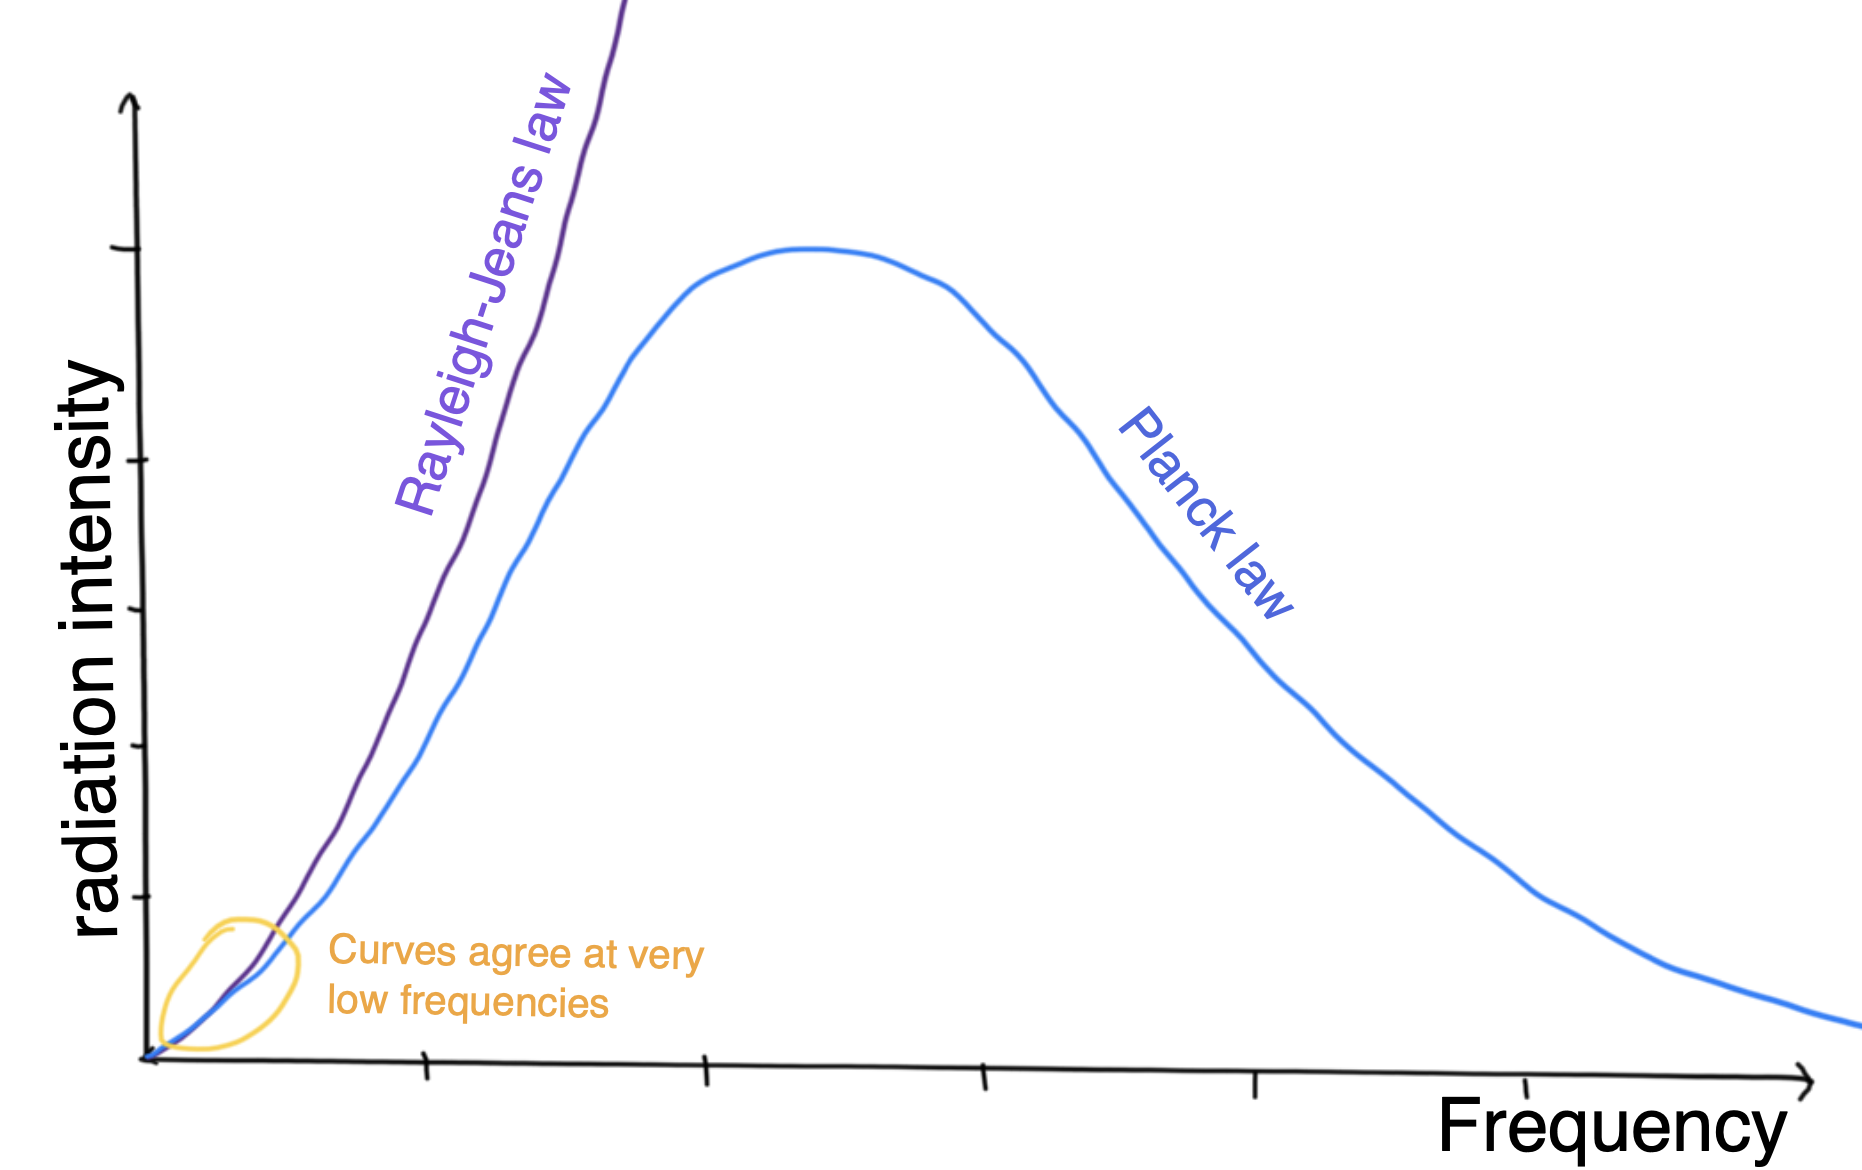
\includegraphics[width=0.7\textwidth]{qm1.png}
\end{center}

\subsection{Photoelectric effect (1905)}
\paragraph{Classical expectation}
Consider a metal surface in a vacuum, which is hit by light with angular frequency \( \omega \).
When the radiation hits the surface of the metal, electrons were emitted.
Classically, we would expect that:
\begin{enumerate}
	\item Since the incident light carries energy $ \propto $ its intensity, increasing the intensity we should have sufficient energy to break the bonds of the electrons with the atoms of the metal.
	\item Since the intensity and frequency are independent, light of any \( \omega \) would eventually cause electrons to be emitted, given a high enough intensity.
	\item The emission rate should be constant.
\end{enumerate}
\begin{center}
    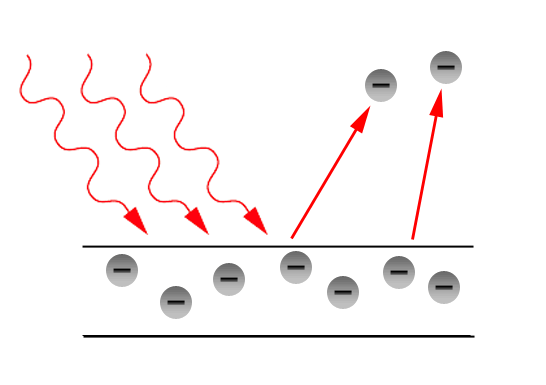
\includegraphics[width=0.7\textwidth]{qm2.png}
\end{center}
\paragraph{Inconsistency with experiment and interpretation}
Experiments showed that
\begin{enumerate}
	\item The maximum energy \( E_{\max} \) of emitted electrons depended on \( \omega \) not $I$. 
	\item Below a given threshold \( \omega_{\min} \), no electron emission.
	\item The emission rate $ \nearrow $ as $ I \nearrow $.
\end{enumerate}
Einstein's explanation for this phenomenon was that 
\begin{enumerate}
    \item The light was \textit{quantised} into small quanta, called \textbf{photons}.
    \item Each carries \( E = \hbar \omega, \mathbf{p}= \hbar \mathbf{k} \).
    \item Each photon could liberate only one electron.
    Thus,
    \[
        E_{\max} = \hbar \omega - \Phi
    \]
    where \( \Phi \) is the binding energy of the electron with the metal aka \textbf{work function}.
    \item $ \nearrow I \Leftrightarrow \nearrow \# \text{ of photons}\Leftrightarrow \nearrow \text{ scattering}\Leftrightarrow \text{higher }e^- \text{ emission rate}$.
\end{enumerate}

\subsection{Compton scattering (1923)}

X-rays were emitted towards a crystal, scattering free electrons.
The X-ray should then be deflected by some angle \( \theta \).

\begin{center}
    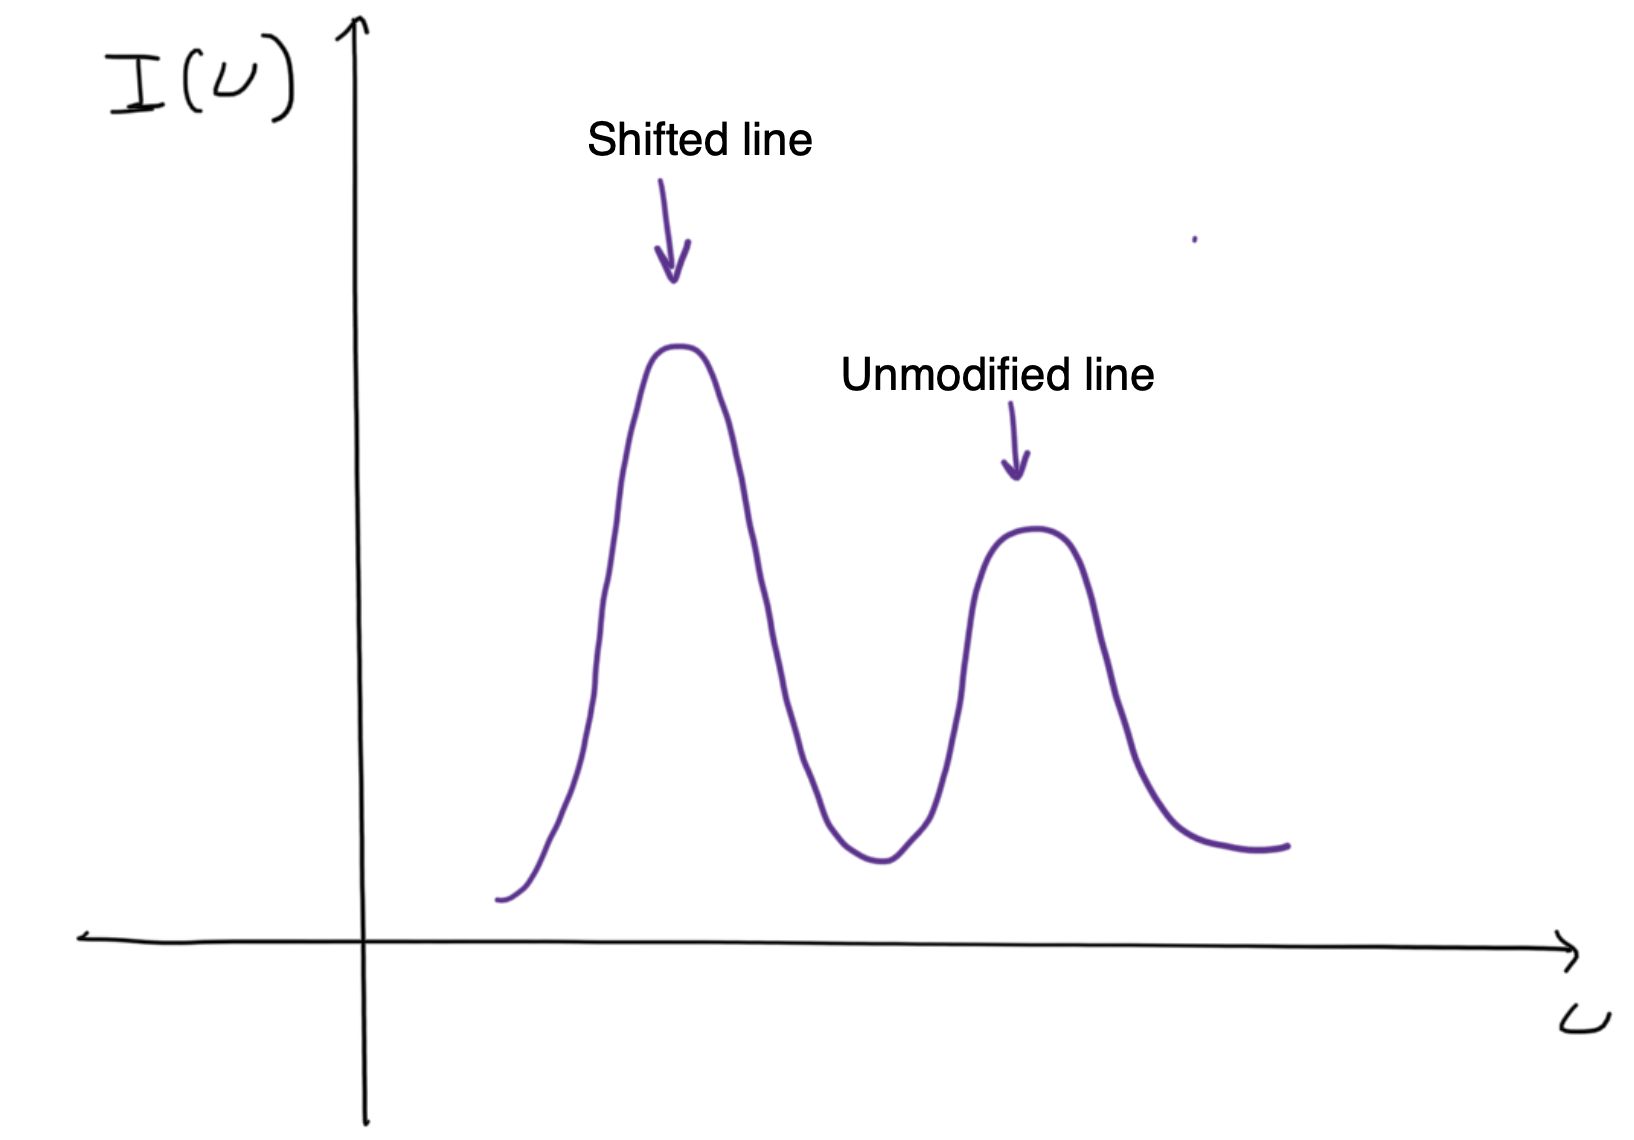
\includegraphics[width=0.5\textwidth]{qm3.png}
    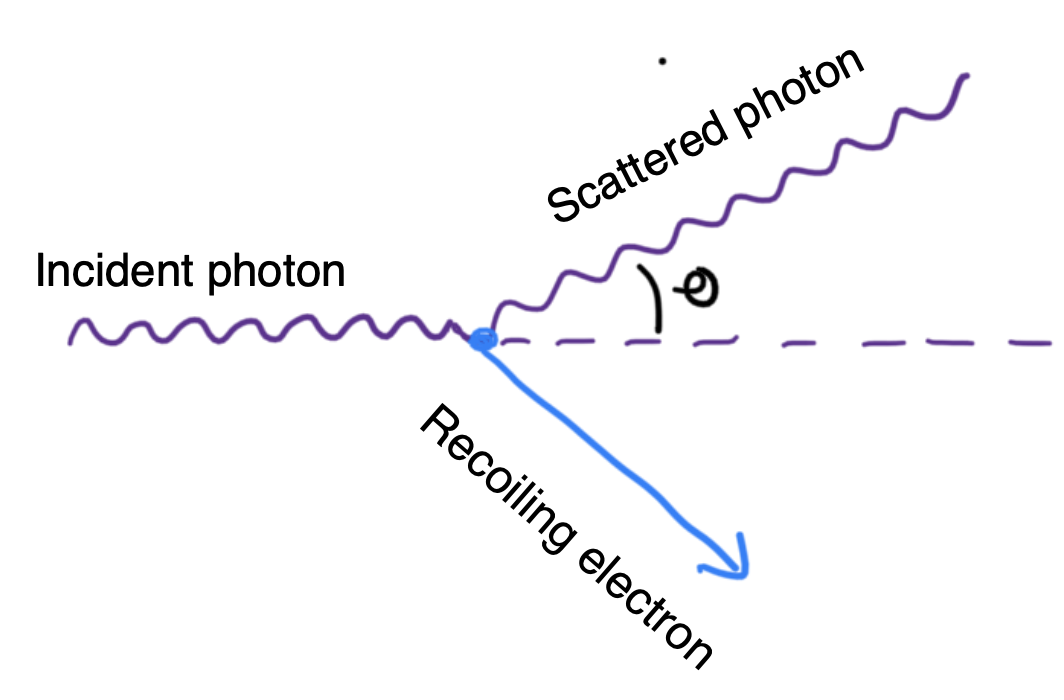
\includegraphics[width=0.45\textwidth]{qm4.png}
\end{center}

Classically, for a given \( \theta \) we would expect that the intensity as a function of \( \omega \) would have a maximum at \( \omega_0 \), the frequency of the incoming X-rays.
This is because we would not expect \( \omega \) to change much after scattering an electron.

However, there was another peak at \( \omega' \), which was dependent on the angle \( \theta \).
In fact, considering the photon and electron as a relativistic system of particles, we can derive (from IA Dynamics and Relativity),
\[
	2 \sin^2 \frac{\theta}{2} = \frac{mc}{\abs{\vb q}} - \frac{mc}{\abs{\vb p}}
\]
where \( \vb p \) is the initial momentum and \( \vb q \) is the final momentum.
Assuming \( E = \hbar \omega \) and \( \vb p = \hbar \vb k \),
\[
	\abs{\vb p} = \hbar \abs{\vb k} = \hbar \frac{\omega}{c}\quad \abs{\vb q} = \hbar \abs{\vb k'} = \hbar\frac{\omega'}{c}
\]
Hence,
\[
	\frac{1}{\omega} = \frac{1}{\omega'} + \frac{\hbar}{mc}(1-\cos\theta)
\]
So the frequency of the outgoing X-ray should have an angular frequency which is shifted from the original.
The expected peak was actually caused by X-rays simply not interacting with the electrons.

\subsection{Atomic spectra}
The Rutherford scattering experiment: shoot \( \alpha \) particles at some thin gold foil.
Most particles travelled through the foil, some were slightly deflected, and some were deflected completely back.
This indicated that the gold foil was mostly comprised of vacuum and there was a high density of positive charge within the atom. 
Which leads to Rutherford's model that electrons would orbit around the nucleus.

\begin{center}
    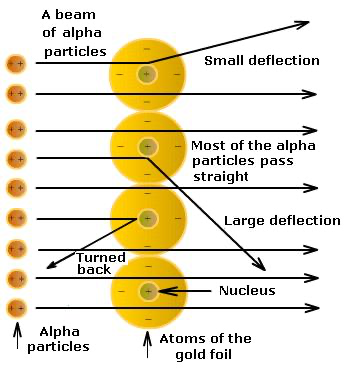
\includegraphics[width=0.5\textwidth]{qm5.png}
\end{center}

However, there were problems with this model:
\begin{enumerate}
	\item If the electrons in orbits moved, they would radiate and lose energy.
	      However if the electrons were static, they would simply collapse and fall into the nucleus.
	\item This model did not explain the atomic spectra, the observed frequencies of light absorbed or emitted by an atom when electrons change energy levels.
\end{enumerate}
The spectra had frequency
\[
	\omega_{mn} = 2 \pi c R_0 \qty(\frac{1}{n^2} - \frac{1}{mc}); \quad m, n \in \mathbb N, m > n
\]
where \( R_0 \) is the Rydberg constant, approximately \( \SI{1e7}{\per\metre} \).

In 1913 Niels Bohr observed that these problems could be resolved in a way consistent with Planck's and Einstein's earlier postulates, if we suppose that the electron orbits of hydrogen atoms are quantised so that the orbital angular momentum takes one of a discrete set of values
\[
L=n \hbar \quad \text { with } \quad n \in \mathbb{N}, n>0 .
\]
\begin{proposition}
    Quantisation of $L \implies $ quantisation of $r,v,E$. 
\end{proposition}
\begin{proof}
    In a circular motion, the angular momentum is given by
\[
L=m_e v r,
\]
we can derive
\[
v \equiv v_n=\frac{n \hbar}{m_e r} .
\]
Coulomn force 
\[
    F_{\text {Coulomb }}=\frac{e^2}{4 \pi \epsilon_0} \frac{1}{r^2}=m_e \frac{v^2}{r} 
\]
So 
\[
    r \equiv r_n=n^2\left(\frac{4 \pi \epsilon_0}{m_e e^2} \hbar^2\right) \equiv n^2 r_0, \quad
        r_0=\frac{4 \pi \epsilon_0 \hbar^2}{m_e e^2} \sim \SI{0.53e-10}{\metre}
\]
$a_0$ is the \textbf{Bohr radius}. Energy is also quantised: 
\[
    E_n=\frac{1}{2} m_e v_n^2-\frac{e^2}{4 \pi \epsilon_0} \frac{1}{r_n}=-\frac{e^2}{8 \pi \epsilon_0 a_0} \frac{1}{n^2}=-\frac{e^4 m_e}{32 \pi^2 \epsilon_0^2 \hbar^2} \frac{1}{n^2} \equiv \frac{E_1}{n^2}
\]
where $ E_1=-\left(e^4 m_e\right) /\left(32 \pi^2 \epsilon_0^2 \hbar^2\right) \sim \SI{-13.6}{eV} $ is the \textbf{groud level}. 
\end{proof}

\begin{center}
    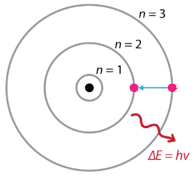
\includegraphics[width=0.3\textwidth]{qm6.png}
\end{center}

Note that 
\[
R_0=\frac{m_e c}{2 \hbar}\left(\frac{e^2}{4 \pi \epsilon_0 \hbar c}\right)^2
\]
agrees well with the experimentally determined values of the Rydberg constant.

\subsection{Wave-like behaviour of particles (1923)}
De Broglie hypothesised that any particle of any mass is associated with a wave with
\[
	\omega = \frac{E}{\hbar}; \quad \vb k = \frac{\vb p}{\hbar}
\]
This hypothesis made sense of the quantisation of electron angular momentum; if the electron lies on a circular orbit then \( 2 \pi r = n \lambda \) where \( \lambda \) is the wavelength of the electron.
However,
\[
	p = \hbar k = \hbar \frac{2 \pi}{\lambda} \implies L = m_e v r = p r = \hbar \frac{2 \pi}{\lambda} \frac{n \lambda}{2 \pi} = n \hbar
\]
Hence the angular momentum must be quantised.
The electron diffraction experiment showed that this hypothesis was true, by showing that electrons behaved sufficiently like waves.
Interference patterns were observed with \( \lambda = \frac{2 \pi}{\abs{\vb k}} = \frac{2 \pi k}{\abs{\vb p}} \) compatible with the De Broglie hypothesis.

\clearpage

\part{Foundations of Quantum Mechanics}
\section{Wavefunctions and probabilistic interpretation}
\subsection{Probabilistic interpretation}

In classical mechanics, a particle is described with \( \vb x, \dot{\vb x} \) or \( \vb p = m \dot{\vb x} \).
In quantum mechanics, it is described by a state \( \psi= \psi(\vb x, t) \) called the wavefunction.

\begin{definition}
    A wavefunction is a function \( \psi(\vb x, t) \colon \mathbb R^3 \to \mathbb C \) that satisfies certain mathematical properties dictated by its physical interpretation.
\end{definition}
\begin{note}
    \( t \) is considered a fixed external parameter, so it is not included in the function's type.
\end{note}

\paragraph{The physical interpretation} is called \textbf{Born's rule.}

\begin{proposition}[Born's rule]
    The probability density for a particle to be at some point \( \vb x \) at \( t \) is given by 
    \[
        \rho(\mathbf{x},t) \propto \left| \psi(\mathbf{x},t) \right| ^2. 
    \]
    The probability that the particle lies in some small volume \( V \) centred at \( \vb x \) is given by 
    \[
        \rho(\vb x, t) \dd{V}.
    \]
\end{proposition}

\paragraph{The mathematical properties} Now we can list the properties explicitly:
\begin{enumerate}
    \item The particle must be somewhere, so the wave function must be \textit{normalisable}, or \textit{square-integrable} in \( \mathbb R^3 \):
    \[
        \int_{\mathbb R^3} \psi^*(\vb x, t) \psi(\vb x, t) \dd{V} = \int_{\mathbb R^3} \abs{\psi(\vb x, t)}^2 \dd{V} = N \in (0, \infty).
    \]
    \item Total probability is 1, which leads to normalised wavefunction
    \[
        \overline{\psi}(\vb x, t) = \frac{1}{\sqrt{N}} \psi(\vb x, t) \iff \int_{\mathbb R^3} \abs{\overline{\psi}(\vb x, t)}^2 \dd{V} = 1.
    \]
    Hence, \( \rho(\vb x,t) = \abs{\overline{\psi}(\vb x,t)}^2 \).
\end{enumerate}

\begin{note}
    \begin{enumerate}
        \item Often we drop the bar and just write wavefunction as $ \psi $, and normalise at the end. 
        \item If $ \widetilde{\psi}(\mathbf{x},t) = e^{i\alpha} \psi(\mathbf{x},t) $ with $ \alpha\in \mathbb{R} $, then $ \left| \widetilde{\psi}(\mathbf{x},t) \right|^2 = \left| \psi(\mathbf{x},t) \right| ^2  $, i.e. $ \psi,\widetilde{\psi} $ are \textit{equivalent states}. 
        \item *We can think of states as arrays in the vector space of wavefunctions.
        We can then describe the equivalence class \( [\psi] \) as the set of all functions \( \phi \) such that \( \phi = \lambda \psi \), for some \( \lambda \in \mathbb C \setminus \qty{0} \), since we must retain the condition that \( \phi \) is normalisable.
    \end{enumerate}
\end{note}

\paragraph{Compare linear algebra to QM} Linear algebra and quantum mechancis have a lot of similarities: 
\begin{center}
\begin{tabular}{cc}
    \toprule 
    \textbf{Linear Algebra} & \textbf{Quantum Mechanics} \\ \midrule
    Vector: $\displaystyle \mathbf{v} = (v_1,\dots,v_n)$ & State $ \psi: \mathbf{x} \mapsto \psi(\mathbf{x},t) $ \\[0.4em] 
    Vector space: $ \mathbb{C}^n $ & Hilbert space: $ L^2( \mathbb{R}^{3}) $ \\[0.4em]  
    Inner product: $ (\mathbf{v},\mathbf{w}) = \mathbf{v}^\dagger \mathbf{w} $ & Inner product: $\displaystyle (\psi,\phi) = \int_{\mathbb{R}^3} \psi^*(\mathbf{x},t)\phi(\mathbf{x},t) \,\mathrm{d}V$ \\[1em]  
    Matrix: $ T = (T_{ij}) $ & Operators: $ \hat{O}: L^2( \mathbb{R}^{3})\to L^2( \mathbb{R}^{3}) $\\
    \bottomrule
\end{tabular}
\end{center}

\subsection{Hilbert space}
The set of all states forms a space, called Hilbert space. 
\begin{definition}
    The set of all square integrable functions in $ \mathbb{R}^3 $ is called \textbf{Hilbert space}, denoted as $ \mathcal{H} \equiv L^2(\mathbb{R}^3) $.
\end{definition}
Check that it is a vector space: 
\begin{proposition}
    $ \mathcal{H} $ is a vector space. Since $ \mathcal{H} \subseteq \mathbb{C}^{\mathbb{R}^3} $, this is equivalent to $ \psi_1,\psi_2\in \mathcal{H} \implies a_1 \psi_1+a_2\psi_2\in \mathcal{H} $, where $ a_1,a_2\in \mathbb{C} $.
\end{proposition}

\begin{proof}
    It suffices to show that: if $\psi_1(\mathbf{x}, t)$ and $\psi_2(\mathbf{x}, t)$ are both normalisable,
    \[
    \int_{\mathbb{R}^3}\left|\psi_1(\mathbf{x}, t)\right|^2 d V=N_1<\infty, \quad \int_{\mathbb{R}^3}\left|\psi_2(\mathbf{x}, t)\right|^2 d V=N_2<\infty,
    \]
    then their linear combination is also normalisable.

    For any two complex number $z_1$ and $z_2$, the triangle inequality states that
    \[
    \left|z_1+z_2\right| \leq\left|z_1\right|+\left|z_2\right|,
    \]
    and
    \[
    \left(\left|z_1\right|-\left|z_2\right|\right)^2 \geq 0 \Rightarrow 2\left|z_1\right|\left|z_2\right| \leq\left|z_1\right|^2+\left|z_2\right|^2 .
    \]
    If we apply these relations for $z_1=a_1 \psi_1$ and $z_2=a_2 \psi_2$, we get
    \begin{align*}
        \int_{\mathbb{R}^3}|\psi(&\mathbf{x}, t)|^2 \dd V =\int_{\mathbb{R}^3}\left|a_1 \psi_1(\mathbf{x}, t)+a_2 \psi_2(\mathbf{x}, t)\right|^2 \dd V \\
        & \leq \int_{\mathbb{R}^3}\left(\left|a_1 \psi_1(\mathbf{x}, t)\right|+\left|a_2 \psi_2(\mathbf{x}, t)\right|\right)^2 \dd V \\
        &=\int_{\mathbb{R}^3}\left(\left|a_1 \psi_1(\mathbf{x}, t)\right|^2+\left|a_2 \psi_2(\mathbf{x}, t)\right|^2+2\left|a_1 \psi_1(\mathbf{x}, t)\right|\left|a_2 \psi_2(\mathbf{x}, t)\right|\right) \dd V \\
        & \leq \int_{\mathbb{R}^3}\left(2\left|a_1 \psi_1(\mathbf{x}, t)\right|^2+2\left|a_2 \psi_2(\mathbf{x}, t)\right|^2\right) \dd V \\
        &=2\left|a_1\right|^2 N_1+2\left|a_2\right|^2 N_2<\infty .\qedhere
    \end{align*}
\end{proof}

\begin{corollary}[Superposition principle]
    If $\psi_1$ and $\psi_2$ correspond to allowed states of a system, then so does the state $\psi$, where
    \[
    \psi=a_1 \psi_1+a_2 \psi_2 \neq 0
    \]
    for arbitrary complex numbers $a_1$ and $a_2$. 
\end{corollary}
This is known as the \textbf{superposition principle}.

\subsection{Inner product}
We can naturally define an inner product on this vector space, in analogy with the finite-dimensional case.

\begin{definition}
    The inner product of two wavefunctions $\psi(\mathbf{x}, t)$ and $\phi(\mathbf{x}, t)$ at a time $t$ is given by
    \[
    (\psi, \phi) \equiv \int_{\mathbb{R}^3} \psi^*(\mathbf{x}, t) \phi(\mathbf{x}, t) \dd V .
    \]
\end{definition}

\begin{theorem}
    The following statements hold.
\begin{enumerate}[(i)]
	\item \( (\psi, \phi) \) exists for all \( (\psi, \phi) \in \mathcal H \)
	\item \( (\psi, \phi^*) = (\phi, \psi) \)
	\item The inner product is antilinear in the first entry, and linear in the second entry
	\item Tor continuous \( \psi \), \( (\psi, \psi) = 0 \) if and only if \( \psi=0 \).
\end{enumerate}
\end{theorem}
\begin{proof}
    (ii)-(iv) are from definition, so we only prove (i). 

    Take $\psi(\mathbf{x}, t)$ and $\phi(\mathbf{x}, t)$. By Cauchy-Schwartz inequality,
    \[
    \left|\int_{\mathbb{R}^3} \psi^*(\mathbf{x}, t) \phi(\mathbf{x}, t) \dd V\right| \leq \sqrt{\int_{\mathbb{R}^3}|\psi(\mathbf{x}, t)|^2 \dd V \int_{\mathbb{R}^3}|\phi(\mathbf{x}, t)|^2 \dd V} .
    \]
    So if both terms on RHS are finite, then also the inner product is finite.
\end{proof}

Using the definition of inner product, we can define (or redefine) a series of important properties of wavefunctions:

\begin{definition}
    \begin{enumerate}
        \item The \textbf{norm} of a wavefunction is $\|\psi\|=\sqrt{(\psi, \psi)}$.
        \item A wavefunction $\psi$ is \textbf{normalised} if $\|\psi\|=1$.
        \item Two wavefunctions $\psi, \phi$ are \textbf{orthogonal} if $(\psi, \phi)=0$.
        \item A set of wavefunctions $\left\{\psi_n\right\}$ is \textbf{orthonormal} is they are normalised and mutually orthogonal:
        \[
        \left(\psi_m, \psi_n\right)=\delta_{m n} .
        \]
        \item A set of wavefunctions $\left\{\psi_n\right\}$ is \textbf{complete} if any other wavefunction in Hilbert space can be expressed as a linear combination of them:
        \[
        \phi=\sum_{n=0}^{\infty} c_n \psi_n
        \]
    \end{enumerate}
\end{definition}

\begin{lemma}
    If the wavefunctions $\left\{\psi_n\right\}$ that form a complete set are also an orthonormal set, the coefficients of $ \phi $ in $ \{\psi_n\} $ are given by:
    \[
    c_n=\left(\psi_n, \phi\right).
    \]
\end{lemma}
\begin{proof}
    \begin{align*}
        \left(\psi_n, \phi\right) &=\left(\psi_n, \sum_{m=0}^{\infty} c_m \psi_m\right) \\
        &=\sum_{m=0}^{\infty} c_m\left(\psi_n, \psi_m\right)=\sum_{m=0}^{\infty} c_m \delta_{m n}=c_n.\qedhere
    \end{align*}
\end{proof}

\section{Time-dependent Schr\"odinger equation (TDSE)}
\subsection{Definition of TDSE}\
\vspace{-1.5em}
\begin{definition}
	The evolution of the wavefunction over time is given by the \textbf{time-dependent Schr\"odinger equation (TDSE)},
	\[
		i\hbar \pdv{\psi}{t} = -\frac{\hbar^2}{2m} \laplacian \psi + U \psi
	\]
	where \( U = U(x) \) is a real potential energy term.
\end{definition}

\begin{remark}
	This equation is a first-order differential equation in \( t \).
	Contrast this to Newton's second law, which is a second-order differential equation in \( t \).
	This implies that we only need a single initial condition \( \psi(x,t_0) \) to determine all future behaviour.
\end{remark}
\begin{remark}
	Note the asymmetry between the spatial and temporal components: there is only a first derivative in time but a second derivative in space.
	This implies that this equation is incompatible with relativity, where time and space must be treated equitably.
\end{remark}
One way to conceptualise the TDSE is by letting \( \psi \) be some wave defined by
\[
	\psi(x,t) = \exp[ i(k \cdot x - \omega t) ]
\]
Then, the De Broglie hypothesis (\( k = p/\hbar, \omega = E/m \)) implies that
\[
	\psi(x,t) = \exp\qty[\frac{i}{\hbar}\qty(p \cdot x - \frac{p^2}{2m}t)]
\]
which is a solution to the TDSE.

\subsection{Conservation of probability}\
\vspace{-1.5em}
\begin{proposition}
    Any TDSE preserves normalization of the wavefunction $\psi$. 
\end{proposition}
\begin{proof}
    We will show that (Recall Born's rule)
    \[
        \frac{\mathrm{d}}{\mathrm{d}t} \int_{\mathbb{R}^3} | \psi(\mathbf{x},t)|^2 \,\mathrm{d}V = 0 \iff \int_{\mathbb{R}^3} | \psi(\mathbf{x},t)|^2 \,\mathrm{d}V = \text{const}.
    \]
    Notice that 
    \begin{align*}
        \frac{\mathrm{d}}{\mathrm{d}t} \int_{\mathbb{R}^3} | \psi|^2 \,\mathrm{d}V &= \int_{ \mathbb{R}^{3}} \frac{\partial }{\partial t}|\psi|^2  \,\mathrm{d}V\\ 
        &=\int_{\mathbb{R}^3} \frac{\partial }{\partial t}(\psi^* \psi)  \,\mathrm{d}V\\ 
        &= \int_{\mathbb{R}^3} \psi^* \frac{\partial \psi}{\partial t} + \psi\frac{\partial \psi^*}{\partial t}   \,\mathrm{d}V. 
    \end{align*}
    By TDSE, 
    \[
        \frac{\partial \psi}{\partial t} = \frac{i\hbar}{2m}\nabla^2 \psi - \frac{i}{\hbar} U \psi,\quad \frac{\partial}{\partial t} \psi^*=-\frac{i \hbar}{2 m} \nabla^2 \psi^*+\frac{i}{\hbar} U \psi^*,
    \]
    so 
    \[
        \frac{\partial}{\partial t}|\psi|^2=\frac{i \hbar}{2 m}\left(\psi^* \nabla^2 \psi-\psi \nabla^2 \psi^*\right)=\nabla \cdot\left[\frac{i \hbar}{2 m}\left(\psi^* \nabla \psi-\psi \nabla \psi^*\right)\right]. 
    \]
    Hence the integral is 
    \begin{align*}
        \int_{ \mathbb{R}^{3}} \frac{\partial }{\partial t}|\psi|^2  \,\mathrm{d}V &= \int_{\mathbb{R}^3} \nabla \cdot\left[\frac{i \hbar}{2 m}\left(\psi^* \nabla \psi-\psi \nabla \psi^*\right)\right] \,\mathrm{d}V\\ 
        &= \int_{\partial V} \frac{i \hbar}{2 m}\left(\psi^* \nabla \psi-\psi \nabla \psi^*\right) \cdot \mathrm{d} \mathbf{S}\\ 
        &= 0 
    \end{align*}
    by divergence theorem, given that $ \psi = 0 $ on $ \partial V $, i.e. $ |\mathbf{x}|\to \infty  $. 
\end{proof}

Recall that for normalized $ \psi $,
\[
    \rho(\mathbf{x},t) = | \psi(\mathbf{x},t)|^2
\]
is the probability density function. 

\begin{proposition}[Conservation of probability]
    We have the following \textit{conservation of probability}
    \[
    \frac{\partial \rho}{\partial t}+\nabla \cdot \mathbf{j}=0,
    \]
    where
    \[
    \mathbf{j}=-\frac{i \hbar}{2 m}\left(\psi^* \nabla \psi-\psi \nabla \psi^*\right).
    \]
\end{proposition}

It is straight from the proof of the previous proposition. $ \mathbf{j} $ is called the \textbf{probability current}. 

\section{Expectation and operators}

Given the wavefunction, we would like to extract some information about the particle it represents, i.e. \textit{observe} or \textit{measure} them. 
\begin{definition}
	An \textbf{observable} is a property of the particle that can be measured.
\end{definition}

In quantum mechanics, each observable is represented by an operator acting on the state \( \psi \).

\subsection{Heuristic interpretation}
From probabilistic interpretation, each measurement is represented by an expectation value of the operator. Expecation value of an observable is the mean of infinite series of measurements performed on particles on the same state. 
\begin{example}
    The measurement on position is given by 
    \[
    \langle x \rangle  = \int_{-\infty}^{\infty} x \left| \psi(x,t) \right| ^2 \,\mathrm{d}x = \int_{-\infty}^{\infty} \psi^*(x,t) x \psi(x,t) \,\mathrm{d}x.
    \]
    Measurement on momentum is 
    \[
        \begin{aligned}
            \langle p\rangle =m \frac{\dd\langle x\rangle}{\dd t}&=m \frac{\dd}{\dd t} \int_{-\infty}^{+\infty} x|\psi(x, t)|^2 \dd x=m \int_{-\infty}^{+\infty} x \frac{\partial}{\partial t}\left(\psi^*(x, t) \psi(x, t)\right) \dd x \\
            &=\frac{i \hbar}{2} \int_{-\infty}^{+\infty} x \frac{\partial}{\partial x}\left(\psi^*(x, t) \frac{\partial \psi(x, t)}{\partial x}-\psi(x, t) \frac{\partial \psi^*(x, t)}{\partial x}\right) \dd x\\ 
            &= \int_{-\infty}^{+\infty} \psi^*(x, t)\left(-i \hbar \frac{\partial}{\partial x}\right) \psi(x, t) \dd x.
        \end{aligned}
    \]
\end{example}
In general, to calculate the expectation value of any quantity $\mathcal{Q}(x, p)$, we simply replace $p$ by $(-i \hbar \partial / \partial x)$ and insert the resulting operator between $\psi^*$ and $\psi$ and integrate over the whole space
\[
\langle\mathcal{Q}(\mathbf{x}, \mathbf{p})\rangle=\int_{\mathbb{R}^3} \psi^* \mathcal{Q}(\mathbf{x},-i \hbar \nabla) \psi \dd V
\]

\subsection{Hermitian operators}
In quantum mechanics, linear transformations are represented by linear operators $\hat{O}$, which act on wavefunctions to produce new wavefunctions of the Hilbert space $\mathcal{H}$.

\begin{definition}
	An \textbf{operator} is a linear map \(\hat{O}: \mathcal H \to \mathcal H \) such that
	\[
		\hat O(a_1 \psi_1 + a_2 \psi_2) = a_1 \hat O(\psi_1) + a_2 \hat O(\psi_2)
	\]
	where \( a_1, a_2 \in \mathbb C, \psi_1, \psi_2 \in \mathcal H \).
\end{definition}

\begin{example}
\begin{itemize}
    \item Finite differential operators
    \[
    \sum_{n=0}^N p_n(x) \frac{\partial^n}{\partial x^n}
    \]
    where the $p_n(x)$ are polynomials. in $x$. Note that this includes the $\hat{p}$ and $\hat{x}$.
    \item the translation operators
    \[
    \hat{S}_a: \quad \psi(x) \rightarrow \psi(x-a)
    \]
    \item the parity operator
    \[
    \hat P: \quad \psi(x) \rightarrow \psi(-x)
    \]
\end{itemize}
\end{example}

\begin{definition}
    The \textbf{Hermitian conjugate} $\hat{O}^{\dagger}$ of an operator $\hat{O}$ is the operator such that
    \[
    \left(\hat{O}^{\dagger} \psi_1, \psi_2\right)=\left(\psi_1, \hat{O} \psi_2\right)
    \]
    for all normalisable wavefunctions $\psi_1, \psi_2 \in \mathcal{H}$.
\end{definition}
From Vectors and Matrices, 
\begin{enumerate}
    \item $\left(a_1 \hat{A}_1+a_2 \hat{A}_2\right)^{\dagger}=a_1^* \hat{A}_1^{\dagger}+a_2^* \hat{A}_2^{\dagger}$,
    \item $(\hat{A} \hat{B})^{\dagger}=\hat{B}^{\dagger} \hat{A}^{\dagger}$.
\end{enumerate}
\begin{definition}
    An operator $ \hat{O} $ is \textbf{Hermitian} if $ \hat{O} = \hat{O}^{\dagger} $.
\end{definition}

Most of the operators we deal with are hermitian: 
\begin{example}
    \begin{itemize}
        \item position
        \[
        \hat{x}: \quad \psi(x, t) \mapsto x \psi(x, t),
        \]
        \item momentum
        \[
        \hat{p}: \quad \psi(x, t) \mapsto-i \hbar \frac{\partial \psi(x, t)}{\partial x} ,
        \]
        \item kinetic energy
        \[
        \hat{T}: \quad \psi(x, t) \mapsto \frac{\hat{p}^2}{2 m} \psi(x, t)=-\frac{\hbar^2}{2 m} \frac{\partial^2 \psi(x, t)}{\partial x^2},
        \]
        \item potential energy
        \[
        \hat{U}: \quad \psi(x, t) \mapsto U(\hat{x}) \psi(x, t)=U(x) \psi(x, t),
        \]
        \item total energy, sum of the kinetic and the potential energies
        \[
        \hat{H}: \quad \psi \mapsto-\frac{\hbar^2}{2 m} \frac{\partial^2}{\partial x^2} \psi(x, t)+U(x) \psi(x, t) .
        \]
        It is often called Hamitonian. 
    \end{itemize}
\end{example}

We will now describe several crucial properties of Hermitian operators.

\begin{theorem}
    \begin{enumerate}[(i)]
        \item The eigenvalues of Hermitian operators are real. 
        \item Eigenfunctions corresponding to different eigenvalues are orthogonal. 
        \item The discrete and continuous sets of eigenfunctions of any Hermitian operator together form a complete orthogonal basis of the physical wavefunctions, i.e. of the normalisable complex-valued wavefunctions $ \psi $. 
    \end{enumerate}
\end{theorem}
\begin{proof}
    See Vectors and Matrices, and Dr Ubiali's notes. 
\end{proof}
\end{document}